\section{Experiments}

\label{sec:experiments}

% PAPER_STUDIO_PARAGRAPH:E-P1

\subsection{Experimental Setup}

We evaluate gpt-5-mini-2025-08-07 on ARC-Challenge and MMLU with deterministic decoding at temperature 0. Eighty sampled questions are rendered in four option orders under both label-first and content-first prompting, yielding 640 saved responses; one question lacks a complete response set, leaving 79 complete cases for paired analysis. Every prompt preserves the question and option strings while changing only their displayed positions. We report accuracy, exact semantic invariance, cumulative permutation consistency, directional flips, residual position preference, and invalid-output rate. Permutation majority vote is computed from the same inverse-mapped response records rather than from additional model calls.

% PAPER_STUDIO_PARAGRAPH:E-P2

\subsection{Main Results}

Table~\ref{tab:main-results} reports the main comparison, and Figure~\ref{fig:planned-results} traces how exact invariance changes as additional option orders are included. On ARC-Challenge, label-first reaches 0.950 accuracy and 0.925 invariance, while content-first reaches 0.925 and 0.875. On MMLU, label-first reaches 0.622 accuracy and 0.487 invariance, whereas content-first reaches 0.654 and 0.615. Permutation majority vote yields 0.925 accuracy on ARC-Challenge and 0.641 on MMLU. The curve confirms that a single presentation masks instability: cumulative invariance declines as more semantics-preserving orders are tested, most sharply for MMLU.

\begin{figure}[htbp]
  \centering
  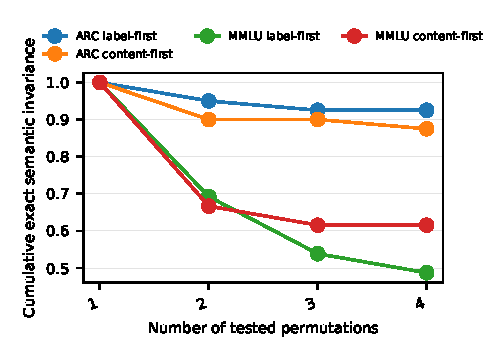
\includegraphics[width=\columnwidth]{fig/permutation_consistency.pdf}
  \caption{Panel a shows four permutation-consistency curves (cumulative exact semantic invariance) across 1 to 4 option permutations for ARC-Challenge and MMLU, using label-first and content-first metrics; invariance declines with permutation count.}
  \label{fig:planned-results}
\end{figure}

\begin{table}[tb]
  \centering
  \small
  \sbox0{\begin{tabular}{lcccc}
    \toprule
    Method & ARC accuracy & ARC invariance & MMLU accuracy & MMLU invariance \\
    \midrule
    Label-first & 0.95 & 0.925 & 0.622 & 0.487 \\
    Content-first & 0.925 & 0.875 & 0.654 & 0.615 \\
    Permutation majority vote & 0.925 & N/A & 0.641 & N/A \\
    \bottomrule
  \end{tabular}}
  \ifdim\wd0>\linewidth\resizebox{\linewidth}{!}{\usebox0}\else\usebox0\fi
  \caption{Measured accuracy and exact semantic invariance across datasets and decision rules.}
  \label{tab:main-results}
\end{table}

% PAPER_STUDIO_PARAGRAPH:E-P3

The results separate task accuracy from response stability. Content-first recovery improves MMLU accuracy by about 3.2 percentage points and invariance by about 12.8 points relative to label-first, but it reduces both quantities on ARC-Challenge. It is therefore not a universal correction for option-order sensitivity. Majority vote also does not dominate the single-order rules: its ARC-Challenge accuracy matches content-first and trails label-first, while its MMLU accuracy lies between them. These dataset-dependent reversals show why reporting only aggregate accuracy or only the best prompting rule would obscure the underlying evaluation fragility.

% PAPER_STUDIO_PARAGRAPH:E-P4

\subsection{Robustness Checks}

We check robustness in two observable dimensions. First, the label-first and content-first analyses reuse identical questions, permutations, and raw responses, so their difference isolates answer recovery rather than a new sample of model behavior. Second, ARC-Challenge and MMLU show qualitatively different magnitudes but both lose exact invariance as more orders are included, ruling out an explanation confined to one benchmark. The conclusions remain those of a reduced-sample pilot: one model, four tested orders, and 79 complete items cannot establish robustness across model families, prompt templates, or all possible permutations.
